\documentclass[11pt, oneside]{book}
\usepackage[utf8]{inputenc}
\usepackage{graphicx}
\usepackage{hyperref}

\usepackage{times}
\usepackage{textcomp}
\usepackage{latexsym}
\renewcommand{\UrlFont}{\ttfamily\small}
\usepackage{graphicx}
\usepackage{adjustbox}

\usepackage{balance}
%% Useful packages
\usepackage{graphicx}
\usepackage{amsmath}
\usepackage{subcaption}
%\usepackage[table,xcdraw]{xcolor}
\usepackage{hyperref}
\usepackage{array}
\usepackage[title]{appendix}
\usepackage{adjustbox}
\usepackage{multirow}
\usepackage{arydshln}
%\usepackage{array}
\usepackage{booktabs}
\usepackage{flushend}
\usepackage{enumitem}
\usepackage{tabularx}
\usepackage{natbib}
\usepackage{xcolor}
\usepackage{amssymb}
\setcitestyle{numbers,open={[},close={]},comma}
\setcounter{secnumdepth}{3} 
\newcommand{\paragraphHd}[1] {\vspace{3pt}\noindent\textbf{#1}}

\newcommand{\method}[1]{HAM$_{\text{\,#1}}$}
\newcommand{\charm}[1]{CHARM$_{\text{\,#1}}$}
\newcommand{\wiki}[1]{Wiki-#1}
\newcommand{\attribute}[1]{\textbf{\emph{#1}}}
\newcommand{\paragraphHdTop}[1] {\noindent\textbf{#1}} % use for first in a series of paragraphHd's
\newcommand{\paragraphHd}[1] {\vspace{3pt}\noindent\textbf{#1}}

\newcommand{\squishlist}{
 \begin{list}{$\bullet$}
  { \setlength{\itemsep}{0pt}
     \setlength{\parsep}{1pt}
     \setlength{\topsep}{1pt}
     \setlength{\partopsep}{0pt}
     \setlength{\leftmargin}{1.5em}
     \setlength{\labelwidth}{1em}
     \setlength{\labelsep}{0.5em} } }

\newcommand{\squishend}{
  \end{list}  }
  
\newcommand{\sig}[1]{#1*}
\newcommand{\nsig}[1]{#1\phantom{*}}
\newcommand{\bsig}[1]{\textbf{#1}*}
\newcommand{\bnsig}[1]{\textbf{#1}\phantom{*}}
\newcommand{\best}[1]{\textbf{#1}}


\usepackage{comment}

\begin{document}

\chapter[PRIDE]{Predicting Relationships in Dialogue Excerpts}

\section*{Abstract}
\label{abstract}

%\ \\%[0.25cm]

\droppedcapital{P}{ersonal} knowledge is a versatile resource that is valuable for a wide range of downstream applications.
Background facts about users can allow chatbot assistants to produce more topical and empathic replies.
In the context of recommendation and retrieval models, personal facts can be used to customize the ranking results for individual users.

A \textit{Personal Knowledge Base}, populated with personal facts, such as demographic information, interests and interpersonal relationships, is a unique endpoint for storing and querying personal knowledge. 
Such knowledge bases are easily interpretable and can provide users with full control over their own personal knowledge, including revising stored facts and managing access by downstream services for personalization purposes.

To alleviate users from extensive manual effort to build such personal knowledge base, we can leverage automated extraction methods applied to the textual content of the users, such as dialogue transcripts or social media posts. Conventional extraction methods specialize on well-structured data, such as biographical texts or encyclopedic articles, which are rare for most people.
In turn, conversational data is abundant but is challenging to process and requires specialized methods for extraction of personal facts.

In our research we address the acquisition of personal knowledge from conversational data. We propose several novel deep learning models for inferring speakers' personal attributes:
\begin{itemize}
    \item Demographic attributes, \textit{age}, \textit{gender}, \textit{profession} and \textit{family status} are inferred by \textbf{HAMs} - hierarchical neural classifiers, based on attention mechanism. HAMs efficiently transfer learn between different types of conversational data and provide interpretable predictions.
    
    \item Long-tailed personal attributes, \textit{hobby} and \textit{profession}, are predicted with \textbf{CHARM} - a zero-shot learning model, overcoming the lack of labeled training samples for rare attribute values. By linking conversational utterances to external sources PRIDE is able to predict attribute values, which it never saw during training.
    
    \item \textit{Interpersonal relationships} are inferred with \textbf{PRIDE} - a hierarchical transformer-based model. To accurately predict fine-grained relationships, PRIDE leverages personal traits of the speakers and the style of conversational utterances.
\end{itemize}

Experiments with various conversational texts, including Reddit discussions and movie scripts, demonstrate the viability of our methods and their superior performance compared to state-of-the-art baselines.

\section{Introduction}

\noindent{\bf Motivation and Problem.} A Personal knowledge base enhanced with the information about the users' interpersonal relationships is practical for many applications. For example, relationship facts in a PKB can be accessed by a personalized chat-bot, which will enable it to make better suggestions for the user (for example, suggesting that the user takes her \textit{child} to the zoo instead of a romantic dinner). Moreover, the speech style of the chat-bot, varying from neutral and official to casual and friendly, can be adjusted based on the relationship between the user and her current interlocutor. Finally, if the conversation happens over the phone, the underlying software can automatically assign categories (family/business/..) for the contact list of the user's interlocutors.

With the ubiquity of social media and online forums, user-generated content is available in abundance. Mining personal knowledge from user-generated content to populate PKBs, or \emph{user profiling}, is a long-standing topic in NLP \cite[e.g.,][]{flekova:ACL16:long,basile:2017,tigunova2019listening}. While users' demographic attributes and interests can be learned from their profile descriptions and posts, interpersonal relationships with other users are rarely mentioned explicitly and may only be inferred from their interactions and conversations.

In this work, we develop an automatic method for predicting fine-grained relationships between two speakers, given their logged conversation history.

\begin{figure}[t!]
\centering
\begin{adjustbox}{width=0.46\textwidth}
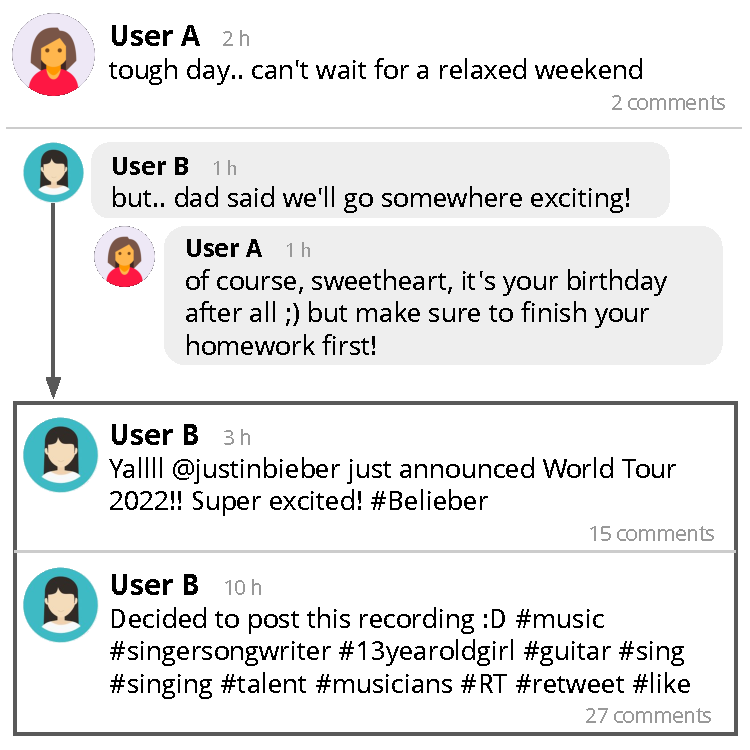
\includegraphics{imgs/conversation_example}
\end{adjustbox}
\caption{Example of 
conversation in social media.}
\label{example_conv}
\end{figure}

Consider the example in Figure~\ref{example_conv}.
From the excerpt of interactions between A and B, the reader can figure out that B is the \textit{child} of A by observing \textit{(i)} the address term `sweetheart', \textit{(ii)} the commanding but soft tone of user A, \textit{(iii)} the reference to the other family member `\textit{dad}', and \textit{(iv)} the context created by the word `\textit{homework}'. Yet, neither of the speakers directly mentions their relationship, making this task difficult for automatic methods 
relying on explicit pattern matching or keyword search.

The relationship information extracted from such conversations, e.g., \textit{<B, child\_of, A>}, can be entered into the PKBs of users A and B. By combining such relationship information with User B's age and personal interests (e.g., \emph{playing guitar, Justin Bieber}) inferable from User B's social media (exemplified in Figure~\ref{example_conv}), 
a system will be able to provide
user A with relevant personalized recommendations for a query ``\textit{birthday present ideas for my daughter}''. 

\paragraphHd{Prior Work and its Limitations.} There has been considerable research on extracting relationships between characters in literary texts such as novels \cite{chaturvedi2016modeling, chaturvedi2017unsupervised}. These methods are inappropriate for conversational data, though, 
which is colloquial and less structured than literary texts. 
Moreover, 
predicting relationships is often  modeled as a binary task of sentiment classification (i.e., person A is positive or negative about person B). 
Prior works on conversational data
are restricted to
small-scale data \cite{yu-etal-2020-dialogue}, or merely handle coarse labels of relationship aspects \cite{rashid2018characterizing,qamar2021relationship}. Most approaches use general models for text classification \cite{chen2020mpdd,jia2020ddrel}, which 
disregard the particularities of
conversational settings. 

\paragraphHd{Approach and Contributions.} We present PRIDE, a 
neural multi-label classifier for \textbf{P}redicting \textbf{R}elationships \textbf{I}n \textbf{D}ialogu\textbf{E}. 
PRIDE makes inference among 12 fine-grained directed relationships (like \emph{child} or \emph{boss}) from conversational data by hierarchically creating utterance representations and combining them with signals on the users' personal attributes (e.g., \textit{age} and \textit{occupation}) and the conversation style (e.g., \textit{intense} or \textit{superficial}).
PRIDE uses BERT \cite{devlin2019bert} to create contextual word embeddings for each utterance, and Transformer encoders \cite{vaswani2017attention} to build conversation representations that preserve information about the sequence and speakers of utterances.

The contributions of this work are: 
\squishlist
\item a method for inferring speakers' relationships from conversational data, which outperforms strong baselines; 
\item an exhaustive analysis of the model's performance. We perform various experiments assessing PRIDE's transfer-learning capabilities and robustness to the varying lengths of the input conversations. Additionally, we conduct ablation studies, proving that all components of the model are essential for the accurate prediction of interpersonal relationships.
\squishend

\section{Related work}

In this section we discuss related work concerning the methods that are used in HAMs. First, we give an overview of the application of neural models utilizing attention mechanism, which is the main building block in our best performing models. Second, we describe the methods for building hierarchical representations of the conversational data. We also refer the reader to Section \ref{back_rel} for a comprehensive overview of the author profiling methods.

\subsection{Neural Models with Attention} 

The role of attention weights has been studied for various neural models, including feed-forward networks \cite{vaswani2017attention}, CNNs, \cite{atten4} and RNNs \cite{bahdanau2014neural}. Recently, neural models enhanced with attention mechanisms have boosted
the results on various NLP tasks \cite{atten1,atten9,atten2}, particularly 
in conversational domain for response generation \cite{atten7, zhang2019recosa}
or spoken language understanding \cite{Chen2016}. 

In response generation task, attention is used to align the context and target utterance representation \cite{atten7}. \citet{zhang2019recosa} extends it with additional self-attention layers for both context and response representations. \citet{Chen2016} uses attention to estimate the relevance of the previous knowledge stored in memory to the input utterances; the response is produced using the attention distribution, calculated by matching each input utterance to the memory vectors.

Transformer \cite{vaswani2017attention} is a state-of-the-art sequence-to-sequence deep learning model based on self-attention mechanism. Transformer is used across various NLP tasks, both as a standalone model and as a part of other neural architectures. In particular, in conversation domain Transformer has been used to produce utterance representations \cite{li2020hierarchical, shan2020contextual}.

\subsection{Hierarchical conversational models} 
\label{ham_hier}

Hierarchical models to represent conversations were introduced in \citet{serban2016building}, which applied RNNs to hierarchically build the representations of utterances and the dialogue context, solving response generation task. \citet{atten8} also decoded conversational responses, introducing attention mechanism into the hierarchical encoder architecture. In \citet{atten8} the utterance and word representations are formed as the attention-weighted averages of the hidden states in word and utterance level RNNs. 

Hierarchical attention models are also utilized for other conversational NLP tasks, such as dialogue state tracking \cite{shan2020contextual} or emotion recognition in conversations \cite{li2020hierarchical, ma2021han}. A common approach is to create word representations with BERT and utterance representations with Transformer encoder \cite{shan2020contextual, li2020hierarchical} or RNN \cite{ma2021han}.

There is also ample research on applying hierarchical attention to speaker attribute prediction. \citet{lynn2020hierarchical} use attention mechanism with the word and utterance representations created by an RNN to predict personality traits of the Facebook users. The study \cite{li2019improving} exploits hierarchical model to predict \textit{age}, \textit{gender} and \textit{location} information of Weibo users.

Compared to most hierarchical models, the architecture of HAMs is more light\hyp{}weight, because it creates speaker representations with an attention mechanism directly, without additionally running an RNN or Transformer models on the attention-weighted words. Thus HAMs are less prone to overfitting and require less computational resources. Regardless of its simplicity, our proposed architecture can still make meaningful predictions in classification tasks with large number of classes, such as \textit{profession} prediction, as opposed to few possible classes in related studies \cite{lynn2020hierarchical, li2019improving}. 



 






\section{Background}
\label{background}

Interactions between people can have multiple fine-grained features, describing various aspects of their communication. For example, interactions can be characterized by attachment style (such as \textit{commitment} or \textit{avoidance}) \cite{qamar2021relationship} or power hierarchy (\textit{subordinate} or \textit{superior}) \cite{prabhakaran2014predicting}. There are ample related social studies researching these characteristics; yet, there is no formal ontology for them \cite{rashid2018characterizing}. One way to organize the features of interpersonal interactions was proposed by \cite{rashid2017dimensions}, defined as \textit{dimensions} of the relationships.

Most of the relationships that we defined for our experiments also have particular interpersonal characteristics. For example, the \textit{enemy} relationship can be described as \textit{competitive} as opposed to \textit{cooperative}; the relationship between \textit{parent} and \textit{child} is in most cases \textit{intimate}. Thus, we find it beneficial to enhance the relationship prediction model with the known features of the speakers' interactions. 

We use the definition of \textit{interpersonal dimensions} \cite{wish1976perceived} of speakers' interactions and relationships, following classification of \citet{rashid2018characterizing}, which we used as an additional input to our model. We note that the discussed interpersonal dimensions are descriptive of the relationship between a particular pair of speakers, but not of the relationship type in general (for example, the interaction between \textit{colleagues} can be both \textit{cooperative} and \textit{competitive}). However, in general any interpersonal dimension can be more or less typical for a relationship type; we use this information to give the model hints about applicable predictions.

\citet{rashid2018characterizing} consider 11 interpersonal dimensions, divided into dimensions of relationships and interactions, as shown in Table \ref{dimensions}. In our model we use all proposed dimensions to provide a comprehensive summary of the relationship's fine-grain characteristics. %For details on each dimension we refer the reader to the original paper \cite{rashid2018characterizing}.
\citet{rashid2018characterizing} also provide a conversational dataset, where every utterance has annotations for each considered interpersonal dimension. We utilize this dataset to pretrain a model for utterance-level dimension classification and create separate representations for each dimension, which are later used in PRIDE.

\begin{table}[t!]
\centering
\begin{adjustbox}{width=0.7\textwidth}
\begin{tabular}{@{}l|ll@{}}
\multirow{4}{*}{relationships} & cooperative vs. noncooperative & equal vs. hierarchical\\ 
 & pleasure vs. work oriented & intense vs. superficial \\ 
 & intimate vs.unintimate & active vs. passive \\ 
 & temporary vs. long term \\ \hline
\multirow{2}{*}{interactions}  & cooperative vs. noncooperative & active vs. passive \\ 
 & concurrent vs. non concurrent & near vs. distant \\                                                          
\end{tabular}
\end{adjustbox}
\caption{Interpersonal dimensions used in PRIDE.}
\label{dimensions}
\end{table}




\section{Methodology}
\label{sec:method}

In this section we describe \textit{Hidden Attribute Models} (HAMs) 
for predicting the values of a given personal attribute using a sequence of utterances made by a speaker.
Formally, given a speaker $S$ and an attribute $P$, our goal is to predict a probability distribution over attribute values $O$ for the attribute based on the speaker's utterances from a dialogue corpus (e.g., a movie script). Each speaker $S$ is associated with a sequence of $N$ utterances $[U_{1}, U_{2}, ..., U_{N}]$ containing $M$ terms each, $U_1 = [U_{1,1}, U_{1,2}, ..., U_{1,M}]$. Each term $U_{n,m}$ is represented as a $d$-dimensional word embedding.

HAMs
can be described in terms of three functions and their outputs:
\begin{enumerate}
\item $f_{utter}$ creates a representation $R^{utter}_n$  of the $nth$ utterance given the terms in the utterance:
\begin{equation}
R^{utter}_n = f_{utter}(U_{n,1}, U_{n,2}, ..., U_{n,M})
\end{equation}
\item $f_{subj}$ creates a speaker representation $R^{subj}$ given the sequence of utterance representations:
\begin{equation}
R^{sp} = f_{subj}(R^{utter}_1, R^{utter}_2, ..., R^{utter}_N)
\end{equation}
\item $f_{obj}$ outputs a probability distribution over attribute values $O$ given the speaker representation:
\begin{equation}
O = f_{obj}(R^{subj})
\end{equation}
Depending on the attribute which value is being predicted, this distribution is used to either make a prediction (for binary attributes, e.g. \textit{gender}) or to produce a ranked list of object values (for multi-class attributes, such as \textit{profession}).
\end{enumerate}

\noindent
In the following sections we describe Hidden Attribute Models by instantiating these functions.

\subsection{Hidden Attribute Models}

\paragraphHdTop{\method{avg}} illustrates the most straightforward way to combine word and utterance representations.
In this model,
\begin{equation}
avg(X) = \sum_{i=1}^{|X|} X_i
\end{equation}
serves as both $f_{utter} $ and $f_{sp}$; the $n$-th utterance representation $R^{utter}_n$ is created by averaging the terms in the $n$-th utterance and the speakert representation $R^{sp}$ is created by averaging the $N$ utterance representations together. Two stacked fully connected layers serve as the function $f_{obj}$,
\begin{equation}
FC(x) = \sigma(Wx+b)
\end{equation}
where $\sigma$ is an activation function and $W$ and $b$ are learned weights.
The full \method{avg} model is then
\begin{equation}
R^{utter}_n = avg(U_n)
\end{equation}
\begin{equation}
R^{subj} = avg(R^{utter})
\end{equation}
\begin{equation}
O = FC_1(FC_2(R^{subj}))
\end{equation}
where $FC_2$ uses a sigmoid activation and $FC_1$ uses a softmax activation function in order to predict a probability distribution over object values.

\paragraphHd{\method{2attn}} extends \method{avg} with two self-attention mechanisms, allowing the model to learn which terms and utterances to focus on for the given predicate. In this model the utterance representations and speaker representations are computed using attention-weighted averages,
\begin{equation}
attn{\text -}avg(X, \alpha) = \sum_{i=1}^{|X|} X_i \alpha_i
\end{equation}
with the attention weights calculated over utterance terms and utterance representations, respectively.
That is, $f_{utter}(X)=attn{\text -}avg(X, \alpha^{term})$ and $f_{so}(X)=attn{\text -}avg(X, \alpha^{utter})$, where
the attention weights for each term in an utterance $U_i$ are calculated as
\begin{equation} \label{eq:attn1}
w^{term}_i = \sigma(W^{term} U_i + b^{term})
\end{equation}
\begin{equation} \label{eq:attn2}
\alpha^{term}_{i,j} = \frac{exp(w^{term}_{i,j})}{\sum_j exp(w^{term}_{i,j})}
\end{equation}
and the utterance representation weights $\alpha^{utter}$ are calculated analogously over $R^{utter}$.
Given these attention weights, the \method{2attn} model is
\begin{equation}
R^{utter}_n = attn{\text -}avg(U_n, \alpha^{term})
\end{equation}
\begin{equation}
R^{sp} = attn{\text -}avg(R^{utter}, \alpha^{utter})
\end{equation}
\begin{equation}
O = FC(R^{sp})
\end{equation}
where $f_{obj}$ function $FC$ uses a softmax activation function as in the previous model.

\paragraphHd{\method{CNN}} considers n-grams when building utterance representations, unlike both previous models that treat each utterance as a bag of words. In this model $f_{utter}$ is implemented with a text classification CNN \cite{cnn} with a ReLU activation function and $k$-max pooling across utterance terms (i.e., each filter's top $k$ values are kept).
A second $k$-max pooling operation across utterance representations serves as $f_{sp}$.
As in the previous model, a single fully connected layer with a softmax activation function serves as $f_{obj}$.

\paragraphHd{\method{CNN-attn}} extends \method{CNN} by using attention to combine utterance representations into the speaker representation.
This mirrors the approach used by \method{2attn}, with $f_{sp}=attn{\text -}avg(X, \alpha^{utter})$ and $\alpha^{utter}$ computed using equations \ref{eq:attn1} and \ref{eq:attn2} as before.
This model uses the same $f_{utter}$ and $f_{obj}$ as \method{CNN}. That is, utterance representations are produced using a CNN with $k$-max pooling, and a single fully connected layer produces the model's output.

\subsection{Training}
All 
HAMs
were trained with gradient descent to minimize a cross-entropy loss. 
We use the Adam optimizer \cite{adam} with its default values and apply an L2 weight decay (2e-7) to the loss.

\section{Experimental setup}

\subsection{Data splitting and preprocessing.} 
For experiments with PRIDE we used Film Relationship (FiRe) dataset, described in Section 3.1.2.
From the input scripts we removed personal names\footnote{
%Based on the list in 
\href{https://catalog.data.gov/dataset/baby-names-from-social-security-card-applications-national-data}{\texttt{\justify https://catalog.data.gov/dataset/baby-names-from-social-\\security-card-applications-national-data}}} and movie-specific words (which we defined as words found in only one movie script), to reduce overfitting to movie domain or genre.

We performed five-fold cross-validation, training the models on three folds and choosing hyperparameter settings according to the performance on 1-fold validation set. We report the results on the remaining 1-fold test set. We arranged the folds so that the sets of movies, where the input character pairs come from, are disjoint. With that as a hard restriction, we tried to maximally balance the label distributions across the folds. For that we created multiple random assignments of movies to folds and chose the one that maximized the balance metrics, which we defined as follows:
\begin{gather*}
    label\_balance = mean([\frac{d_l}{S_l} \mbox{ for l in labels}]), \\
    d_l = \max_{i}s^i_l - \min_{i}s^i_l, 
\end{gather*}
where $S_l$ denotes the number of pairs for the label l in the whole dataset, and $s^i_l$ denotes the number of pairs for the label $l$ in fold $i$.


\subsection{Model setup and evaluation metrics}

We fine-tuned a pretrained BERT model (bert-base-uncased) to create word embeddings. To produce interpersonal dimension embeddings, we train BERT on the labeled data from \citet{rashid2018characterizing} on each dimension separately, resulting in 768-dimensional representations.

We gathered the data about speakers' ages by crawling \url{imdb.com} for the ages of the corresponding actors in the year the film/series was made. To create age embeddings we calculate the age difference (\emph{diff}) between the speakers and assign it to one of the predefined \emph{diff} bins. We set \emph{diff} bins to be [(-inf; -13], [-12; -6], [-5; -1], [0; 4], [5; 11], [12; +inf]] (a negative age difference means that speaker B is younger than speaker A).

\paragraphHd{Training mechanism.} PRIDE is trained in two steps: first we train the model without external representations (age difference and interpersonal dimensions). The pretrained base model checkpoint is then used in full PRIDE to train external representations' embeddings and classification layer (the weights of the base model stay frozen).

We trained the model with Binary Cross Entropy loss. During training we oversampled the under-represented labels. We perform grid search to tune the following hyperparameters: training epoch, learning rate (we use different learning rates for BERT and the rest of the model), word and utterance aggregation (among \textit{max}, \textit{average} and \textit{attention}).
We perform multi-label classification by predicting all labels with a score over a threshold, which we treat as a hyperparameter.

\paragraphHd{Evaluation metrics.} We compute macro-averaged multilabel precision, recall and F1 score as evaluation metrics. During grid search we optimized F1 score of the performance on the development set.

\subsection{Baselines.}
 We compare the performance of PRIDE with the following baselines:
 \squishlist
     \item \textbf{RNN} is a BiLSTM \cite{graves2005framewise} architecture adapted by \citet{welch2019look}, which was trained on short context windows. Before each utterance a special token ('\textlangle ME\textrangle' or '\textlangle OTHER\textrangle') is prepended to represent the speaker.
     \item \textbf{HAM}, described in Chapter 3. To allow multiple relationship predictions we trained \method{2attn} for multi-label classification using Binary Cross-Entropy loss. HAMs are designed to process the utterances from a single speaker; for the experiments in this chapter we did not change the architecture of \method{2attn}, which was trained on the input from both speakers without incorporating any speaker information.
     \item \textbf{BERT$_{conv}$} for sequence classification \cite{lu2020improving} runs on the concatenation of utterances divided by a $[\textrm{SEP}]$ symbol and segment embeddings corresponding to the speaker of each utterance. The sequences of utterances greater than the allowed input length are cropped.
     \item \textbf{BERT$_{ddrel}$} 
     \cite{jia2020ddrel} 
     produces the relationship label ranking for each dialogue snippet in a movie; the final scores for pair-level labels through the whole conversation history is the sum of MRRs of the labels from scenes' predictions.
 \squishend


\section{Results and Discussion}
\label{results}


\subsection{Main Findings}
\label{findings}

In Tables \ref{tab:model-comparison-profession}, \ref{tab:model-comparison-profession}, \ref{tab:model-comparison-age} and \ref{tab:model-comparison-family} we report results for HAMs and the baselines on all datasets (MovieChAtt, PersonaChat and RedDust) for all considered attributes (\textit{profession}, \textit{gender}, \textit{age} and \textit{family status}).
In the tables the results marked with * significantly differ from 
the best performing method (highlighted with bold font)
with $p < 0.05$ as measured by a paired t-test (MRR) or McNemar's test (Acc and AUROC).

\begin{table}[th!] \sffamily
\centering
\small
\begin{adjustbox}{width=0.8\textwidth,center}
\begin{tabular}{@{}lcc|cc|cc@{}}
\toprule
 & \multicolumn{6}{c}{\textbf{profession}} \\
\cmidrule(lr){2-7} 
\multirow{3}{*}{\textbf{Models}} & \multicolumn{2}{c|}{\textbf{MovieChAtt}} & \multicolumn{2}{c|}{\textbf{PersonaChat}} & \multicolumn{2}{c}{\textbf{RedDust}} \\ 
\cmidrule(lr){2-3} \cmidrule(lr){4-5} \cmidrule(lr){6-7} 
 & \multicolumn{1}{c}{MRR} & \multirow{2}{*}{AUROC} & \multicolumn{1}{c}{MRR} & \multirow{2}{*}{AUROC} & \multicolumn{1}{c}{MRR} & \multirow{2}{*}{AUROC} \\
 & micro / macro &  & micro / macro &  & micro / macro & & 
\midrule
%Pattern oracle    & 0.21* / 0.20* & - & - & - & ? & ? & 0.67 & - & - & - & ? & - \\ 
%\hdashline
Embedding sim.    & \sig{0.22} / \sig{0.14} & \sig{0.60} & \sig{0.30} / \sig{0.25} & \sig{0.63} & \sig{0.15} / \sig{0.13} & \sig{0.59}  \\
Logistic reg.     & \sig{0.46} / \sig{0.20} & \sig{0.76} & \sig{0.81} / \sig{0.77} & \sig{0.58} & \sig{0.13} / \sig{0.19} & \nsig{0.57}  \\ 
MLP               & \bnsig{0.47} / \nsig{0.20} & \nsig{0.75} & \sig{0.86} / \sig{0.77} & \nsig{0.97} & \nsig{0.46} / \nsig{0.23} & \nsig{0.78}  \\
\midrule
N-GrAM \cite{basile:2017} & \sig{0.21} / \sig{0.16} & \sig{0.62} & \sig{0.83} / \nsig{0.83} & \nsig{0.88} & \nsig{0.17} / \nsig{0.26} & \sig{0.64}  \\
W2V-C \cite{pietro:ACL15} & \sig{0.25} / \sig{0.13} & \sig{0.74} & \nsig{0.59} / \nsig{0.46} & \nsig{0.89} & \sig{0.27} / \sig{0.17} & \sig{0.74}  \\
CNN \cite{bayot:MOD17} & \sig{0.19} / \sig{0.20} & \sig{0.66} & \sig{0.77} / \sig{0.77} & \sig{0.81} & \sig{0.26} / \sig{0.24} & \sig{0.76}  \\
\midrule
\method{avg}      & \sig{0.39} / \sig{0.37} & \sig{0.81} & \sig{0.86} / \sig{0.91} & \sig{0.98} & \sig{0.34} / \sig{0.22} & \sig{0.82} \\
\method{CNN}      & \nsig{0.42} / \nsig{0.37} & \nsig{0.83} & \bnsig{0.96} / \bnsig{0.94} & \bnsig{0.99} & \sig{0.36} / \sig{0.37} & \sig{0.86} \\ 
\hdashline
\method{CNN-attn} & \nsig{0.43} / \bnsig{0.50} & \bnsig{0.85} & \nsig{0.90} / \nsig{0.93} & \bnsig{0.99} & \bnsig{0.51} / \nsig{0.40} & \bnsig{0.9}  \\
\method{2attn}    & \nsig{0.39} / \nsig{0.34} & \nsig{0.84} & \nsig{0.94} / \nsig{0.93} & \bnsig{0.99} & \nsig{0.43} / \bnsig{0.42} & \nsig{0.89}  \\
\bottomrule
\end{tabular}
\end{adjustbox}
\caption{Comparison of 
models on all datasets for \emph{profession} attribute.}
\label{tab:model-comparison-profession}
\end{table}
\begin{table}[th!]\sffamily
\centering
\small
\begin{adjustbox}{width=0.65\textwidth,center}
\begin{tabular}{@{}lcc|cc|cc@{}}
\toprule
 & \multicolumn{6}{c}{\textbf{gender}} \\
\cmidrule(lr){2-7}
\multirow{3}{*}{\textbf{Models}} & \multicolumn{2}{c|}{\textbf{MovieChAtt}} & \multicolumn{2}{c|}{\textbf{PersonaChat}} & \multicolumn{2}{c}{\textbf{RedDust}}  \\ 
\cmidrule(lr){2-3} \cmidrule(lr){4-5} \cmidrule(lr){6-7} 
 & Acc & AUROC & Acc & AUROC & Acc & AUROC \\
\midrule
Embedding sim.    & \sig{0.52} & \sig{0.54} & \nsig{0.49} & \nsig{0.50} & \sig{0.61} & \sig{0.60} \\
Logistic reg.     & \nsig{0.59} & \nsig{0.62} & \nsig{0.86} & \nsig{0.93} & \sig{0.69} & \sig{0.75} \\ 
MLP                & \sig{0.57} & \sig{0.60} & \nsig{0.80} & \nsig{0.87} & \nsig{0.71} & \nsig{0.77} \\
\midrule
N-GrAM \cite{basile:2017}  & \nsig{0.57} & \nsig{0.58} & \nsig{0.86} & \nsig{0.87} & \sig{0.66} & \sig{0.71} \\
W2V-C \cite{pietro:ACL15} & \nsig{0.62} & \nsig{0.66} & \sig{0.73} & \sig{0.80} & \sig{0.64} & \sig{0.73} \\
CNN \cite{bayot:MOD17} & \nsig{0.60} & \nsig{0.60} & \sig{0.72} & \sig{0.73} & \sig{0.61} & \sig{0.61} \\
\midrule
\method{avg}      & \nsig{0.72} & \nsig{0.82} & \nsig{0.79} & \nsig{0.87} & \bnsig{0.86} & \nsig{0.92} \\
\method{CNN}     & \nsig{0.75} & \bnsig{0.85} & \nsig{0.95} & \bnsig{0.99} & \bnsig{0.86} & \sig{0.93} \\ 
\hdashline
\method{CNN-attn} & \bnsig{0.77} & \nsig{0.84} & \bnsig{0.96}  & \nsig{0.97}  & \nsig{0.85} & \bnsig{0.94} \\
\method{2attn}   & \nsig{0.69} & \nsig{0.77} & \nsig{0.94} & \nsig{0.98} & \nsig{0.80} & \nsig{0.91} \\
\bottomrule
\end{tabular}
\end{adjustbox}
\caption{Comparison of 
models on all datasets for \emph{gender} attribute.}
\label{tab:model-comparison-gender}
\end{table}


We do not report results for the \textit{pattern oracle} baseline as we evaluated this baseline solely on the MovieChAtt dataset, because the oracle essentially replicates the way we labeled persona descriptions and posts in the PersonaChat and RedDust datasets, respectively.
The pattern oracle baseline yields 0.21/0.20 micro/macro MRR for \textit{profession}, 0.67 accuracy for \textit{gender}, and 0.41/0.40 micro/macro MRR for \textit{age}. HAMs significantly outperform this baseline, indicating that identifying explicit mentions of attribute values is insufficient in our dialogue setting.

HAMs outperform the distantly supervised models (i.e., \textit{embedding similarity}, \textit{logistic regression} and \textit{Multilayer Perceptron (MLP)}) in the vast majority of cases.
MLP and logistic regression perform best in several occasions for \textit{profession} and \textit{age} attributes when micro MRR is considered. However, their macro MRR scores fall behind HAMs, showing that HAMs are better at dealing with 
multi-valued attributes having skewed distribution.
The low performance of these distantly supervised methods may be related to their strong assumption that every sequence of four utterances contains information about the attribute being predicted.

Comparing with baselines from prior work, HAMs significantly outperform N-GrAM \cite{basile:2017} in many cases,
suggesting that representing utterances using word embeddings, instead of merely character and word n-grams, is important for this task. 
Using neural clusters (W2V-C) as features for the classification task \cite{pietro:ACL15} works quite well for the \textit{age} attribute, where different `topics' may correlate with different age categories (e.g. `video game' for \textit{teenager} and `office' for \textit{adult}).
However, W2V-C is often significantly worse for the \textit{profession}, \textit{gender}, and \textit{family status} attributes, which may be caused by similar discriminative words (e.g., `husband'/`wife' for \textit{gender}) being clustered together in the same topic.
The CNN baseline \cite{bayot:MOD17} is significantly worse than the best method in the majority of cases. Furthermore, it generally performs substantially worse than \method{CNN}, further illustrating the advantage of aggregating utterances within the model.

In general, \method{avg} performs worse than the other HAMs%\footnote{
%For the sake of brevity we neither instantiate nor report results for LSTM-based HAMs, such as $f_{utter}=\text{\textit{LSTM}}$ and $f_{subj}=attn{\text -}avg$ or $f_{subj}=\text{\textit{LSTM}}$. These models were unable to outperform \method{avg}, with the best variant obtaining a micro MRR of only 0.31 after grid search (profession attribute on MovieChAtt; Table \ref{tab:model-comparison-profession-gender}). This is in line with recent results suggesting that RNNs are not ideal for identifying semantic features \cite{tang2018self}.}
, demonstrating that simple averaging is insufficient
for representing utterances and speakers.
In most cases \method{CNN} performs slightly worse than \method{CNN-attn}, demonstrating
the value of exploiting an attention mechanism to combine speaker's utterances.

\method{CNN-attn} and \method{2attn}  
achieve the strongest performance across attributes, with \method{CNN-attn} generally performing better.
\method{CNN-attn} performs particularly well on the \textit{gender} and \textit{family status} attributes, where detecting bigrams may yield an advantage. For example, \method{2attn} places high attention weights on terms like `family' and `girlfriend' where the previous term may be a useful signal (e.g., `my family' vs. `that family').

The gap between the baselines and HAMs is often smaller on PersonaChat compared with the other two datasets, illustrating the simplicity of crowdsourced dialogues as compared to movie scripts or Reddit discussions. This is also supported by the fact that the maximum metrics on PersonaChat are much higher. There are several factors that may be responsible for this: \textit{(1)} the dialogues in PersonaChat were created by the crowdworkers with the goal of using predefined personal facts, which often leads to those facts being stated in a straightforward manner (e.g., saying ``My job is a writer'' given the persona description sentence ``I am an writer''); \textit{(2)} PersonaChat utterances are much shorter 
and there are far fewer utterances per character (i.e., a maximum of 4 in PersonaChat vs. a minimum of 20 in MovieChAtt), leading to a higher density of information related to attributes; and \textit{(3)} the same persona descriptions in PersonaChat are used across multiple separate dialogue sessions, giving models an opportunity to learn specific personas.

For the sake of brevity we neither instantiate nor report results for LSTM-based HAMs, such as $f_{utter}=\text{\textit{LSTM}}$ and $f_{subj}=attn{\text -}avg$ or $f_{subj}=\text{\textit{LSTM}}$. These models were unable to outperform \method{avg}, with the best variant obtaining a micro MRR of only 0.31 after grid search (profession attribute on MovieChAtt; Table \ref{tab:model-comparison-profession}). This is in line with recent results suggesting that RNNs are not ideal for identifying semantic features \cite{tang2018self}.

\begin{table}[] \sffamily
\centering
\small
\begin{adjustbox}{width=0.45\textwidth}
\begin{tabular}{@{}lcc|cc@{}}
\toprule
& \multicolumn{4}{c}{\textbf{family status}} \\
\cmidrule(lr){2-5}
\multirow{2}{*}{\textbf{Models}} & \multicolumn{2}{c|}{\textbf{PersonaChat}} & \multicolumn{2}{c}{\textbf{RedDust}} \\ 
\cmidrule(lr){2-3} \cmidrule(lr){4-5} 
 & Acc & AUROC & Acc & AUROC \\
\midrule
Embedding sim.    & \sig{0.41} & \sig{0.49} & \sig{0.42} & \sig{0.47} \\
Logistic reg.     & \sig{0.75} & \sig{0.84} & \nsig{0.71} & \nsig{0.74} \\ 
MLP               & \nsig{0.70} & \nsig{0.80} & \sig{0.62} & \sig{0.60} \\
\midrule
N-GrAM \cite{basile:2017} & \nsig{0.85} & \nsig{0.86} & \sig{0.45} & \sig{0.47} \\
W2V-C \cite{pietro:ACL15} & \sig{0.74} & \sig{0.82} & \nsig{0.70} & \nsig{0.78} \\
CNN \cite{bayot:MOD17} & \nsig{0.74} & \nsig{0.74} & \nsig{0.69} & \nsig{0.69} \\
\midrule
\method{avg}      & \nsig{0.80} & \nsig{0.91} & \nsig{0.67} & \nsig{0.72} \\
\method{CNN}      & \bnsig{0.93} & \bnsig{0.99} & \sig{0.52} & \sig{0.62} \\ 
\hdashline
\method{CNN-attn} & \nsig{0.92} & \nsig{0.98} & \bnsig{0.70} & \bnsig{0.78} \\
\method{2attn}    & \nsig{0.88} & \nsig{0.94} & \nsig{0.64} & \nsig{0.67} \\
\bottomrule
\end{tabular}
\end{adjustbox}
\caption{Comparison of 
models on all datasets for \emph{family status} attribute.}
\label{tab:model-comparison-family}
\end{table}

\begin{table}[]\sffamily
\centering
\small
\begin{adjustbox}{width=0.55\textwidth}
\begin{tabular}{@{}lcc|cc@{}}
\toprule
& \multicolumn{4}{c}{\textbf{age}} \\
\cmidrule(lr){2-5}
\multirow{3}{*}{\textbf{Models}} & \multicolumn{2}{c|}{\textbf{MovieChAtt}} & \multicolumn{2}{c}{\textbf{RedDust}} \\ 
\cmidrule(lr){2-3} \cmidrule(lr){4-5} 
 & \multicolumn{1}{c}{MRR} & \multirow{2}{*}{AUROC} & \multicolumn{1}{c}{MRR} & \multirow{2}{*}{AUROC} \\
 & micro / macro &  & micro / macro &  \\
\midrule
%Pattern oracle    & \sig{0.41} / \sig{0.40} & - & ? / ? & - \\ 
%\hdashline
Embedding sim.    & \sig{0.45} / \sig{0.45} & \sig{0.61} & \sig{0.55} / \sig{0.44} & \sig{0.56} \\
Logistic reg.     & \sig{0.65} / \sig{0.49} & \nsig{0.76} & \bnsig{0.80} / \nsig{0.61} & \nsig{0.87} \\ 
MLP               & \sig{0.64} / \sig{0.48} & \nsig{0.83} & \nsig{0.78} / \nsig{0.48} & \nsig{0.88} \\
\midrule
N-GrAM \cite{basile:2017} & \nsig{0.69} / \nsig{0.47} & \nsig{0.85} & \sig{0.48} / \sig{0.53} & \sig{0.55} \\
W2V-C \cite{pietro:ACL15} & \nsig{0.67} / \nsig{0.45} & \nsig{0.86} & \nsig{0.75} / \nsig{0.51} & \nsig{0.88} \\
CNN \cite{bayot:MOD17} & \sig{0.66} / \sig{0.62} & \nsig{0.83} & \sig{0.68} / \sig{0.65} & \sig{0.79} \\
\midrule
\method{avg}      & \sig{0.62} / \nsig{0.59} & \sig{0.76} & \nsig{0.67} / \nsig{0.67} & \sig{0.77} \\
\method{CNN}      & \sig{0.73} / \bnsig{0.63} & \nsig{0.84} & \sig{0.73} / \sig{0.61} & \sig{0.89} \\ 
\hdashline
\method{CNN-attn} & \nsig{0.73} / \nsig{0.60} & \bnsig{0.86} & \nsig{0.79} / \bnsig{0.68} & \bnsig{0.90} \\
\method{2attn}    & \bnsig{0.74} / \nsig{0.6} & \nsig{0.85} & \nsig{0.72} / \nsig{0.6} & \nsig{0.82} \\
\bottomrule
\end{tabular}
\end{adjustbox}
\caption{Comparison of
models on all datasets for \emph{age} attribute.}
\label{tab:model-comparison-age}
\end{table}


\subsection{Study on word embeddings}
In Section \ref{findings} we represented terms using embeddings from a word2vec skip-gram model trained on Google News \cite{embed1}.
In this study we compare the Google News embeddings with word2vec embeddings trained on Reddit posts, GloVe \cite{pennington2014glove} embeddings trained on Common Crawl, and GloVe embeddings trained on Twitter. We also consider $ELMo$ \cite{Peters:2018}, a contextualized embedding model. To capture semantic variations, this model creates a contextualized character-based representation of words using a bidirectional language model. We use AllenNLP's small ELMo model\footnote{https://allennlp.org/elmo} trained on the 1 Billion Word Benchmark of news crawl data from WMT 2011 \cite{41880}. 


\begin{table}[h!]
\centering
\small
\begin{adjustbox}{width=0.7\textwidth,center}
\begin{tabular}{@{}l@{\hskip 1\tabcolsep}l@{}c@{\hskip 1\tabcolsep}cc@{\hskip 1\tabcolsep}c@{}}
\toprule
\multirow{3}{*}{\textbf{Model}} & \multirow{3}{*}{\textbf{Corpus}} & \multicolumn{2}{c}{\textbf{\method{CNN-attn}}} & \multicolumn{2}{c}{\textbf{\method{2attn}}} \\
 \cmidrule(lr){3-4} \cmidrule(lr){5-6}
 &  & MRR & AU- & MRR & AU- \\
 &  & micro / macro & ROC & micro / macro & ROC\\
 \midrule
 %\multicolumn{5}{l}{\textbf{word2vec (skip-gram)}} \\
word2vec & Google News & 0.42 / \textbf{0.44} & 0.77 & 0.39 / 0.37 & \textbf{0.83} \\
(skip-gram) & Reddit & \textbf{0.43} / 0.37 & \textbf{0.82} & \textbf{0.50} / 0.37 & \textbf{0.83} \\
 \midrule
 %\multicolumn{5}{l}{\textbf{GloVe}} \\
 \multirow{2}{*}{GloVe} & Common Crawl & 0.40 / 0.37 & 0.76 & 0.40 / \textbf{0.39} & 0.82 \\
 & Twitter & 0.39 / 0.35 & 0.67 & 0.36 / 0.34 & 0.81 \\
 %\multicolumn{5}{l}{\textbf{ELMo}} \\
 \midrule
 ELMo & WMT News & 0.38 / 0.32 & 0.76  & 0.37 / 0.37 & 0.83 \\
\bottomrule
\end{tabular}
\end{adjustbox}
\caption{Comparison of embedding models trained on different datasets, for identifying \textit{profession} attribute.
% on MovieChAtt dataset.
}
\label{emb_tab}
\end{table}

Given the higher model variance on the \textit{profession} attribute on MovieChAtt, we restrict the study to this attribute and dataset. We evaluated the two best performing HAMs, i.e., \method{CNN-attn} and \method{2attn}. Table \ref{emb_tab} shows the results obtained with the various embedding methods trained on different corpora.
The difference in performance does not greatly vary across embedding models and corpora, with Google News embeddings performing best in terms of macro MRR and Reddit embeddings performing best in terms of micro MRR.
Despite their strong performance on some NLP tasks, the ELMo contextualized embeddings do not yield a performance boost for any method or metric.
We view this observation as an indicator that the choice of term embedding method is not very significant for this task compared to the method used to combine terms into an utterance representation.


\subsection{Ablation study}

We performed an ablation study in order to determine the performance impact of the HAMs' components.
As in the previous section, we restrict this study to the inference of the \textit{profession} attribute on MovieChAtt dataset. 
Ablation results for \method{2attn} using cross validation on the training set are shown in Table \ref{tab4}.
Replacing either representation function (i.e., $f_{utter}$ or $f_{subj}$) with an averaging operation reduces performance, as shown in the last two lines. Attention on utterance representations ($R^{utter}$) is slightly more important in terms of MRR, but both types of attention contribute to \method{2attn}'s performance.
Similarly, removing both types of attention corresponds to \method{avg}, which consistently underperforms \method{2attn} in Tables \ref{tab:model-comparison-profession}, \ref{tab:model-comparison-gender}, \ref{tab:model-comparison-age} and \ref{tab:model-comparison-family}.


\begin{table}[th!]
\centering
\small
\begin{tabular}{@{}lcc@{}}
\toprule
                         & \multicolumn{1}{c}{MRR} & \multirow{2}{*}{AUROC} \\
                         & micro / macro &  \\
                         \midrule
%\method{CNN-attn} & ? / ? & ? \\
%$-$ attention on $R^{utter}$ & ? / ? & ? \\
\method{2attn}           & \textbf{0.57} / \textbf{0.42} & \textbf{0.84} \\
$-$ attention on terms       & 0.49 / 0.40 & 0.81 \\
$-$ attention on $R^{utter}$ & 0.48 / 0.34 & 0.82 \\
\bottomrule
\end{tabular}
\caption{Ablation study for the \textit{profession} attribute.}
\label{tab4}
\end{table}

Removing attention from \method{CNN-attn} yields \method{CNN}, which consistently performs worse than \method{CNN-attn} in Table \ref{tab:model-comparison-profession}, \ref{tab:model-comparison-gender}, \ref{tab:model-comparison-age} and \ref{tab:model-comparison-family},
supporting the observation that attention is important for performance on our task.
Intuitively, attention provides a useful signal because it allows the model to focus on only the terms containing important information about an attribute.

\begin{figure*}[th!]
 \centering
 \begin{subfigure}{.9\textwidth}
   \centering
   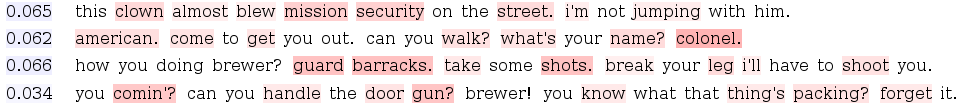
\includegraphics[scale=0.43]{pics/military.png}
   \caption{\textit{profession}: military personnel}
   \label{fig:att-profession}
 \end{subfigure}
 \\[8pt]
 \begin{subfigure}{.9\textwidth}
   \centering
   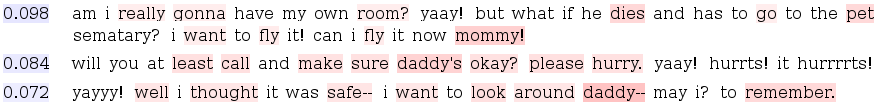
\includegraphics[scale=0.43]{pics/child.png}
   \caption{\textit{age} (category): child}
   \label{fig:att-age}
 \end{subfigure}
\vspace*{-0.3cm}
\caption{Attention visualization for \textit{profession} and \textit{age} attributes on MovieChAtt.}
\label{fig:att-profession-age}
\end{figure*}

\begin{figure*}[th!]
 \centering
 \begin{subfigure}{.9\textwidth}
   \centering
   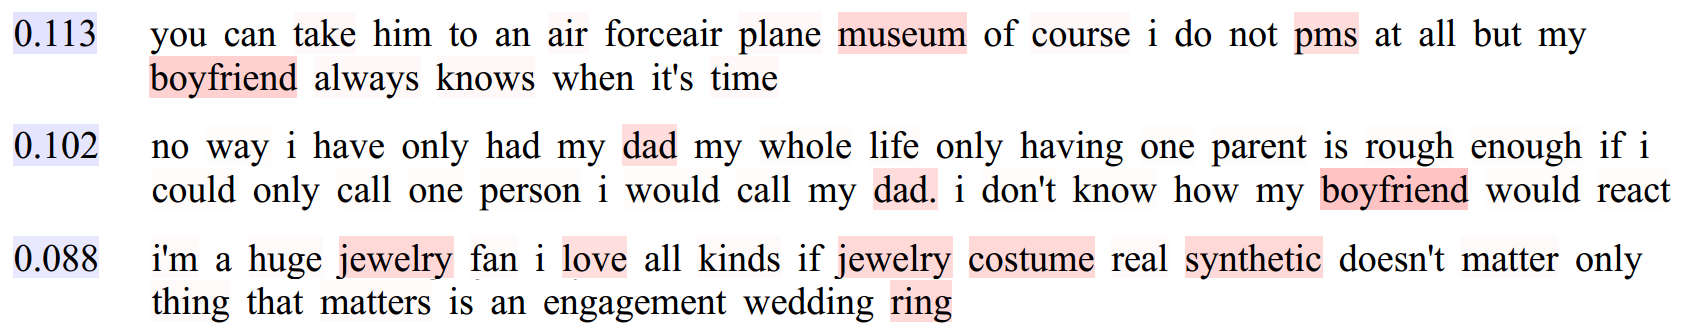
\includegraphics[scale=0.17]{pics/gender_att.png}
   \caption{\textit{gender}: female}
   \label{fig:att-gender}
 \end{subfigure}
 \\[8pt]
 \begin{subfigure}{.9\textwidth}
   \centering
   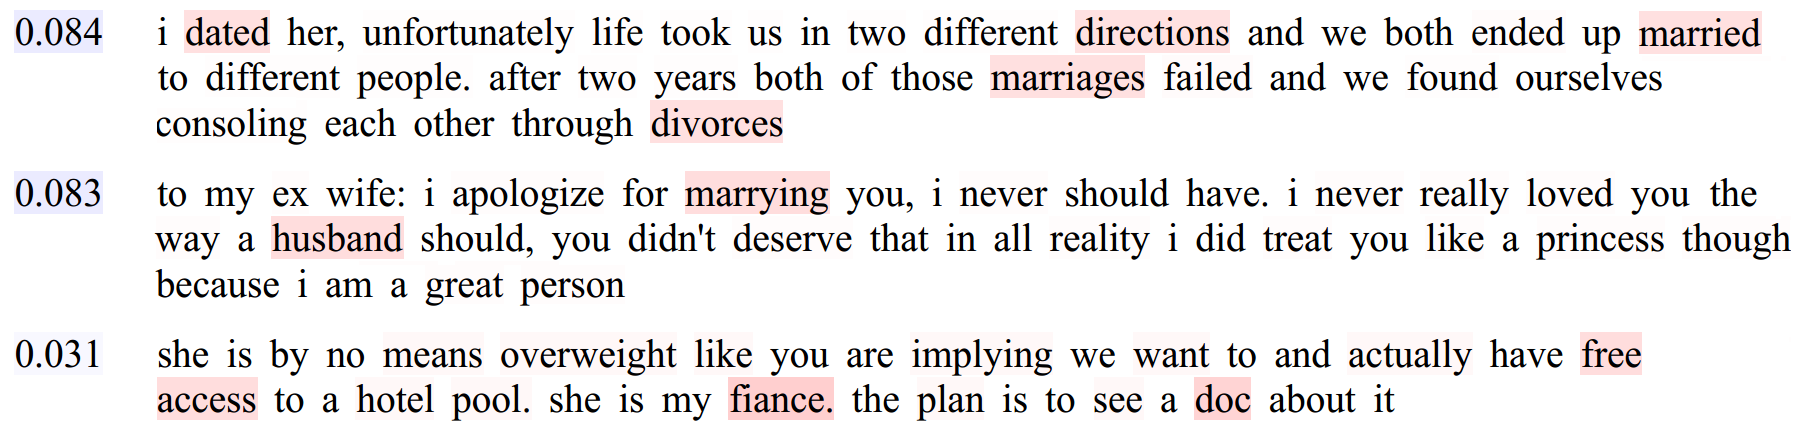
\includegraphics[scale=0.17]{pics/family_att.png}
   \caption{\textit{family status}: married}
   \label{fig:att-family}
 \end{subfigure}
\vspace*{-0.3cm}
\caption{Attention visualization for \textit{gender} and \textit{family status} attributes on RedDust.}
\label{fig:att-gender-family}
\end{figure*}


\subsection{Case study on attention weights}

In order to illustrate the types of terms the models are looking for, we display \method{2attn}'s term and utterance weights for 
\textit{profession} and \textit{age} attributes (on the MovieChAtt dataset) in Figure \ref{fig:att-profession-age}, as well as \textit{gender} and \textit{family status} attributes (on RedDust) in Figure \ref{fig:att-gender-family}.
While \method{2attn} is 
%sometimes
often outperformed by \method{CNN-attn}, this model is more interpretable because individual terms are considered in isolation.
%Note that all these dialogue snippets come from the specific
%datasets in our experiments, partly from fictional
%conversations.
%Some are skewed and biased, and not representative
%for the envisioned downstream applications.

When predicting \textit{military personnel} as the \textit{profession} (Figure \ref{fig:att-profession}), the model focuses on military terms such as \textit{mission}, \textit{guard}, \textit{barracks}, and \textit{colonel}.
When predicting \textit{child} as the \textit{age category} (Figure \ref{fig:att-age}), on the other hand, the model focuses on terms a child is likely to use, such as \textit{pet}, \textit{mommy}, and \textit{daddy}.
According to Reddit posts, \textit{female} gender is suggested by terms such as \textit{boyfriend}, \textit{pms} and \textit{jewelry} (Figure \ref{fig:att-gender}). Meanwhile, \textit{married} users were identified through terms such as \textit{dated}, \textit{fiance} and \textit{divorces}, along with obvious terms like \textit{marrying} and \textit{marriages} (Figure \ref{fig:att-family}). 
These examples illustrate how the model is able to infer a speaker's attribute by aggregating signals across utterances.

In addition to looking at specific utterances, we investigated which terms the model is strongly associating with a specific attribute. To do so, we computed attribute value probabilities for each term in the corpus, and kept the top terms for each attribute value. The results using \method{2attn} are shown in Table \ref{tab6}, which is divided into words that appear informative (top section) and words that do not (bottom section). In the case of informative words, there is a clear relationship between the words and the corresponding profession. 
Many of the uninformative words appear to be movie-specific, such as names (e.g., xavier, leonard) and terms related to a \textit{waiter's} role in a specific movie (e.g., rape, stalkers). Reducing the impact of setting-specific signals like this is one direction for future work.

\begin{table}[t]
\centering
\small
%\begin{adjustbox}{width=0.475\textwidth,center}
\begin{tabular}{@{}l@{\hskip 0.5\tabcolsep}l@{}}
\toprule
\textbf{profession} & \textbf{significant words} \\
\midrule
\textit{scientist} & characteristics, theory, mathematical, species, changes \\
\textit{politician} & governors, senate, secretary, reporters, president \\
\textit{detective} & motel, spotted, van, suitcase, parked \\
\textit{military personnel} & captured, firepower, guard, soldiers, attack \\
\midrule
\textit{student} & playing, really, emotional, definitely, unbelievable \\
\textit{photographer} & xavier, leonard, collins, cockatoo, burke \\
\textit{waiter} & rape, stalkers, murdered, overheard, bothering \\
\bottomrule
\end{tabular}
%\end{adjustbox}
\caption{Top-5 words from \method{2attn} characterizing each profession.
}
\label{tab6}
\end{table}

\vspace{-5pt}
\subsection{Insights on transfer learning}

To investigate the robustness of our trained HAMs,
we tested the best performing models (i.e., \method{2attn} and \method{CNN-attn})
on a transfer learning task between our datasets. 
Specifically, we leveraged user-generated social media text (RedDust posts) available in abundance to train the models and subsequently performing inference on the speech-based dialogues (MovieChAtt and PersonaChat). 
We report the results in Tables \ref{tab:transfer-learning-reddit-moviechatt} and \ref{tab:transfer-learning-reddit-personachat} respectively.

While the scores on PersonaChat are low compared to those in Tables \ref{tab:model-comparison-gender}, \ref{tab:model-comparison-profession} and \ref{tab:model-comparison-family}, the HAMs' performance on MovieChAtt is often comparable with the baselines' performance in Tables \ref{tab:model-comparison-gender}, \ref{tab:model-comparison-profession}, \ref{tab:model-comparison-age} and \ref{tab:model-comparison-family}.
This difference may be caused by the fact that PersonaChat is a smaller, more synthetic dataset, as discussed in Section \ref{findings}.

On MovieChAtt with the \textit{profession} attribute, both HAMs match the performance of all six baselines in terms of macro MRR. Similarly, \method{2attn} matches the performance of five of the six baselines on the \textit{gender} attribute (accuracy), and \method{CNN-attn} matches the performance of four of the six baselines on the \textit{age} attribute (macro MRR). The methods do not perform as well in terms of micro MRR, which may be due to the substantially different attribute value distributions between datasets.
Particularly for the \textit{profession} attribute, the lower performance can be explained by missing training instances  for certain professions in the RedDust dataset, such as \textit{astronaut} or \textit{monarch}. 
Improving HAMs' transfer learning performance is a direction for future work.


\begin{table}[t]
\centering
\small
\begin{adjustbox}{width=0.9\textwidth,center}
\begin{tabular}{@{}lc@{}cc@{\hskip 1\tabcolsep}cc@{}c@{}}
\toprule
\multirow{3}{*}{\textbf{Models}} & \multicolumn{2}{c}{\textbf{profession}\vspace{3pt}} & \multicolumn{2}{c}{\textbf{gender}} & \multicolumn{2}{c}{\textbf{age}} \\
\cmidrule(lr){2-3} \cmidrule(lr){4-5} \cmidrule(lr){6-7}
 & \multicolumn{1}{c}{MRR} & \multicolumn{1}{c}{\multirow{2}{*}{AUROC}} & \multicolumn{1}{c}{\multirow{2}{*}{Acc}} & \multicolumn{1}{c}{\multirow{2}{*}{AUROC}}  & \multicolumn{1}{c}{MRR} & \multicolumn{1}{c}{\multirow{2}{*}{AUROC}}  \\
 & \multicolumn{1}{c}{micro / macro} & &  & & \multicolumn{1}{c}{micro / macro} & \\
\midrule
\Tstrut \method{CNN-attn}     & 0.19 / 0.18 & 0.58 & 0.56 & 0.58 & \textbf{0.57} / \textbf{0.54} & \textbf{0.69} \\ 
\method{2attn}                & \textbf{0.21} / \textbf{0.21} & \textbf{0.67} & \textbf{0.61} & \textbf{0.64} & 0.45 / 0.41 & 0.45 \\
\bottomrule
\end{tabular}
\end{adjustbox}
\caption{Transfer learning performance of pre-trained RedDust models on MovieChAtt.}
\label{tab:transfer-learning-reddit-moviechatt}
\end{table}



\begin{table}[t]
\centering
\small
%\begin{adjustbox}{width=0.475\textwidth,center}
\begin{tabular}{@{}lcccccc@{}}
\toprule
\multirow{3}{*}{\textbf{Models}} & \multicolumn{2}{c}{\textbf{profession}\vspace{3pt}} & \multicolumn{2}{c}{\textbf{gender}} & \multicolumn{2}{c}{\textbf{family status}} \\
\cmidrule(lr){2-3} \cmidrule(lr){4-5} \cmidrule(lr){6-7} 
 & \multicolumn{1}{c}{MRR} & \multicolumn{1}{c}{\multirow{2}{*}{AUROC}} & \multicolumn{1}{c}{\multirow{2}{*}{Acc}} & \multicolumn{1}{c}{\multirow{2}{*}{AUROC}}  & \multicolumn{1}{c}{\multirow{2}{*}{Acc}} & \multicolumn{1}{c}{\multirow{2}{*}{AUROC}} \\
 & \multicolumn{1}{c}{micro / macro} &  &  &  &  & \\
\midrule
\Tstrut \method{CNN-attn}     & 0.20 / 0.16 & 0.58 & \textbf{0.52} & 0.50 & \textbf{0.74} & \textbf{0.74} \\
\method{2attn}                & \textbf{0.21} / \textbf{0.18} & \textbf{0.71} & 0.51 & \textbf{0.54} & 0.62 & 0.64 \\
\bottomrule
\end{tabular}
%\end{adjustbox}
\caption{Transfer learning performance of pre-trained RedDust models on PersonaChat.}
\label{tab:transfer-learning-reddit-personachat}
\end{table}

\subsection{Profession misclassification study}
In this section we investigate common misclassifications on the MovieChAtt dataset for the \textit{profession} attribute, which is the most challenging attribute with the most possible values.
A confusion matrix for \method{2attn} is shown in Figure \ref{matrix}.
Dotted lines indicate several
interesting misclassifications: \textit{policemen} are often confused with \textit{detectives} and \textit{special agents} (red line); \textit{scientists} are confused with \textit{astronauts} (yellow line), because sci-fi films often feature characters who arguably serve in both roles; and a \textit{child} is often labeled as a \textit{student} or a \textit{housewife} (green line) because they sometimes use similar terms (e.g., `school' is used by both children and students, and `mommy' is used by both children and housewives).
Finally, 
many occupations are confused with \textit{criminal}, which is the most common profession in MovieChAtt.


\begin{figure}[t]
\centering
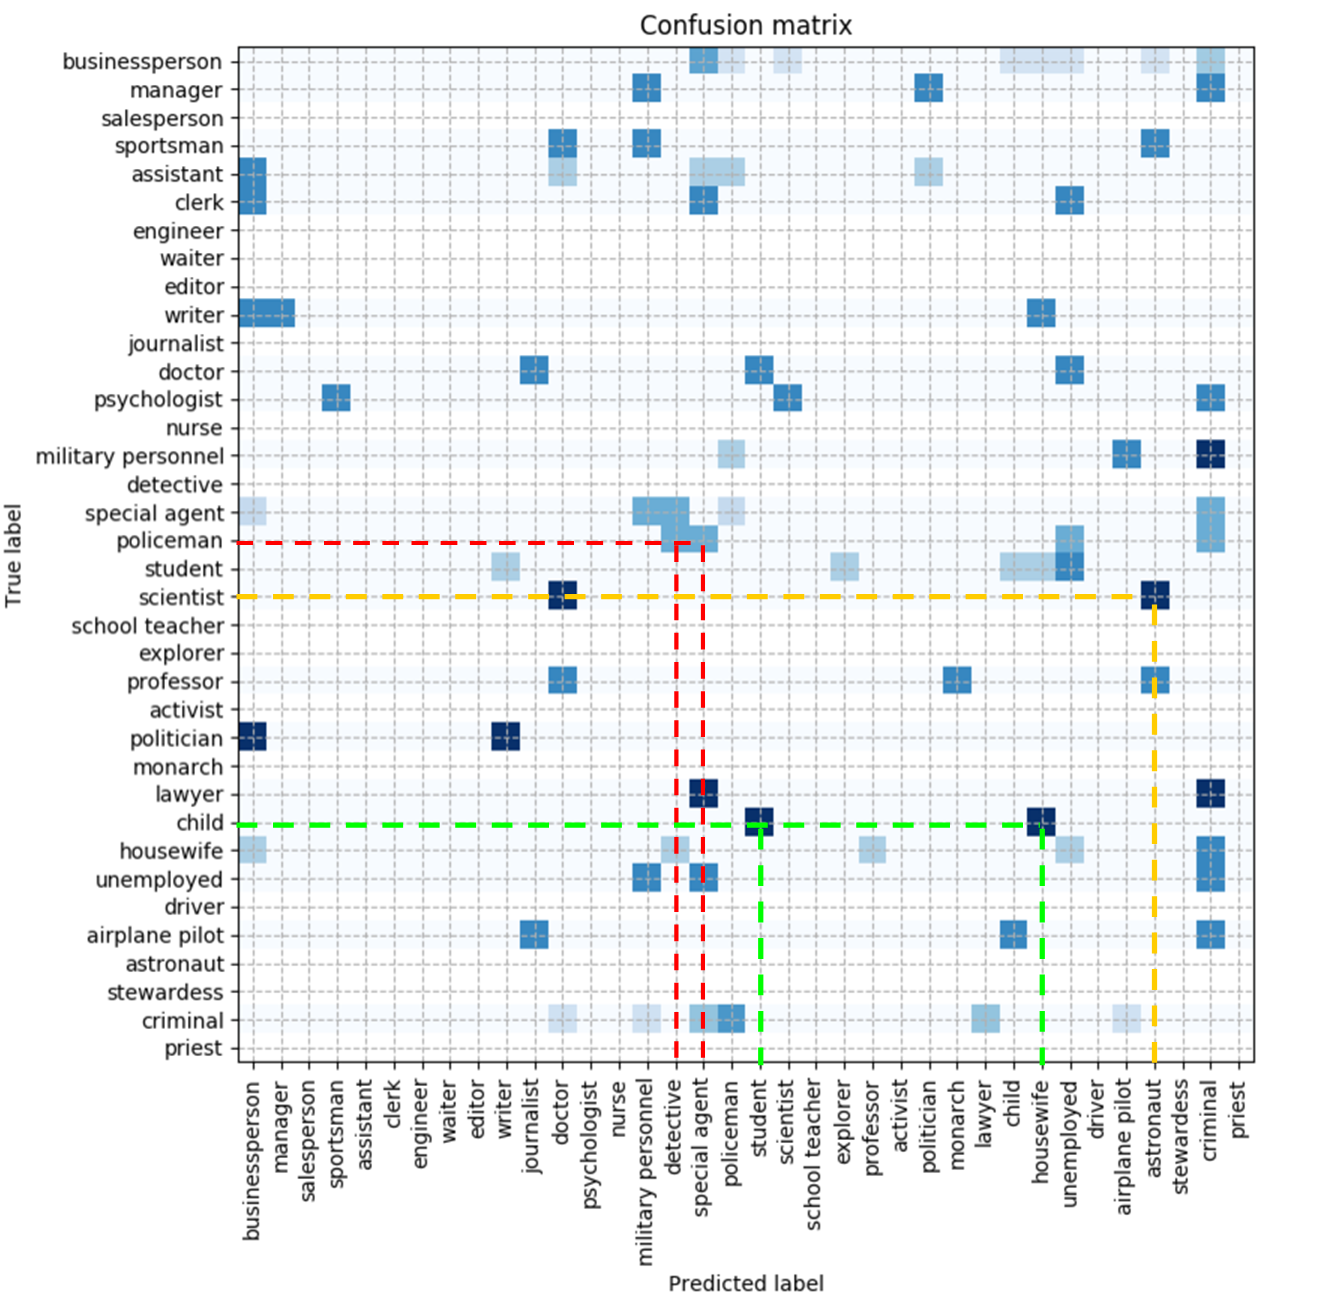
\includegraphics[width=0.7\textwidth]{pics/conf_new.png}
\vspace*{-0.3cm}
\caption{Confusion matrix computed with \method{2attn}. True positives are not shown. Darker squares indicate more misclassifications.}
\label{matrix}
\end{figure}



%%%%%
% Transfer learning confusion matrix (was in original HAM paper)
%
%To further compare the performance of the model on direct and transfer learning tasks we computed the confusion matrix for \method{2attn} trained on the Reddit dataset and using MovieChAtt as the test corpus. Interesting misclassifications include the following: artistic professions (\textit{actor}, \textit{painter}, \textit{musician}, \textit{director}) are often mixed up (red lines); \textit{banker} is confused with \textit{manager} (green lines); \textit{policeman} and \textit{airplane pilot} are confused with \textit{military personnel} (purple lines); and \textit{stewardess} is often confused with \textit{nurse} as they both are related to caring and serving tasks (yellow line).

%\begin{figure}[t]
%\centering
%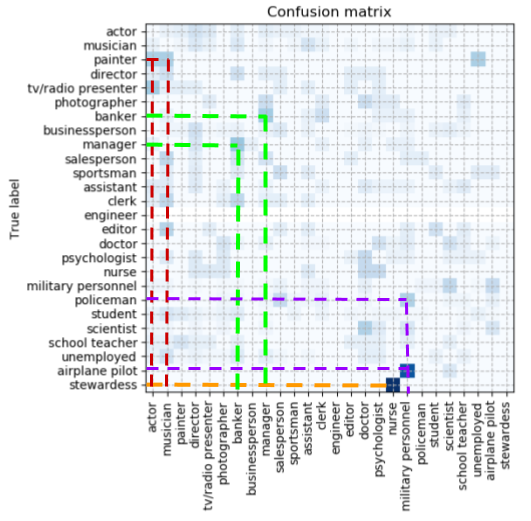
\includegraphics[width=0.75\textwidth]{pics/conf_transfer_crop.png}
%\vspace*{-0.3cm}
%\caption{Confusion matrix of Reddit$_{\text{train}}$ $\rightarrow$ %MovieChAtt$_{\text{test}}$ computed with \method{2attn}. True positives are not shown. %Darker squares indicate more misclassifications.}
%\label{matrix-reddit}
%\end{figure}



\section{Conclusion}

We presented PRIDE, a model for inferring fine-grained relationships from conversations. To our best knowledge, PRIDE is the first model to predict \textit{directed, multilabel} speakers' relationships. PRIDE leverages the hierarchical dialogue structure to efficiently handle lengthy conversational history. The novelty of our architecture is the additional signals of speakers' demographics and speech style, which significantly improve relationship prediction.

PRIDE outperforms state-of-the-art baselines and demonstrates effective transfer learning on different types of dialogue data. %In ablation experiments we demonstrate that the proposed architecture improves the model's predictions. 
PRIDE is designed to perform inference on long conversational sequences; however, we experimentally show PRIDE's ability to make accurate predictions for shorter interactions too. 

To support future work on this topic, we created and released the largest labeled collection of relationships in conversations, which improves over existing datasets by including directed multilabel relationships.

\subsection{Discussion}

In this subsection we discuss several limitations of the current work and propose directions for further improvements of PRIDE:

\begin{itemize}
    \item \textbf{Leveraging other types of conversational data.} Inferring relationships in real-life user conversations is the use case motivating our research. Thus, we find it important to evaluate PRIDE's transfer learning capabilities to other conversational datasets to ensure that it can generalize. Our choice of the dataset was constrained by the complexity of labeling dialogues with relationship labels; we leave it for future work to obtain more diverse relationship datasets (for example, social media interactions or telephone transcripts).
    
    \item \textbf{Improving performance on directed relationships.} Predicting asymmetric relationships has been overlooked in the prior works; yet accurately distinguishing them is important for practical applications. For instance, an intelligent assistant can recommend completely different items, depending of whether the user is asking for a birthday present suggestions for her \textit{parent} or her \textit{child}. Thus, we find it necessary to further improve PRIDE's performance on asymmetric relationships.
    
    \item \textbf{Incorporating more personal attributes.} In our experiments we showed that prediction of interpersonal relationships can benefit from adding speakers' attributes. We find it interesting to experiment on adding other personal information, such as \textit{occupation} or \textit{ethnicity}.

    \item \textbf{Joint prediction of personal attributes and interpersonal relationships.} The current version of PRIDE supports incorporating precomputed ground truth information about the speakers' ages. In the scenario when personal attribute labels are not available, one option is to use a predictive model (such as HAM) to provide such information on the fly. Joint training of the relationship and speakers' attribute prediction models could improve their performance, as relationships and personal attributes are interdependent.

    \item \textbf{Considering multispeaker conversations.} The current dataset used in experiments with PRIDE was limited to uninterrupted dialogue spans between two characters. This limitation was due to the difficulty of distinguishing the addressee of an utterance when more than 2 speakers are present. In real life people often interact in a group, thus considering only speaker pairs will result in losing useful cues for predictions. Therefore, extension of the current model to handle multi-speaker conversations should be further investigated.
    %Therefore, we find it important to investigate the ways the current model can be extended to handle multi-speaker dialogues.

    
\end{itemize}

%The last research direction can also be generalized to the other models discussed in the current thesis. For instance, the people who communicate are often in the same age group and = have the same \textit{hobbies} (if they are friends) or \textit{professions} (if they are colleagues). We highlight simultaneous predictions of personal attributes and relationships using speaker network as a compelling future research direction.

\bibliographystyle{abbrvnat}
\bibliography{bibliography}

\end{document}
